\chapter{CubeSat Design}

	Für die Realisierung einer ADR-Mission liegt der Fokus zunächst bei dem Entwurf eines geeigneten CubeSats. Infolgedessen wird in diesem Kapitel ein bestehendes Konzept \cite{Lettau.} anhand der Software QuSAD (SQL-Based CubeSat Analyse and Design Tool QuSAD) analysiert und gegebenenfalls optimiert. Zuvor wird ein Einblick in das Programm gegeben und durch eine anschließende Beschreibung des angenommenen Entwurfs erfolgt abschließend die Budgetplanung. Letztlich wird mittels der Budgets eine Auswertung des Designs bezüglich seiner Effizienz durchgeführt. Bei Bedarf werden Verbesserungen in Erwägung gezogen. Demnach kann ein zielführendes Missionsdesign bestimmt und bewertet werden.
		
		\section{QuSAD}
			
			\subsection{Einführung in die Software}
	\hfill\emph{(Valentina Dietrich)}\\
	
		Die Software QuSAD (SQL-Based CubeSat Analyse and Design Tool) besteht aus einem SQL-Segment und einem MatLab Segment. Die SQL-Datenbank ist die Haupteingabequelle für das Entwerfen eines CubeSats und kategorisiert die CubeSat-Komponenten. Durch die wissenschaftliche Version können die COTS-Komponenten mit vordefinierten Parametern eingepflegt werden. Zusätzlich können auch individuelle Komponenten mit veränderbaren Parametern mittels der praxis Version hinzugefügt werden. Für das Abrufen der Komponententabelle aus der SQL-Datenbank wird MatLab verwendet. Dies wird durch mehrere grafische Benutzeroberflächen (GUI) realisiert und ermöglicht dem Benutzer eigene Satellitenzusammenstellungen. Neben dem CubeSat Design können Budget-Analysen von Masse, Volumen, Energie, Preis und Verlinkung durch zur Verfügung stehenden Werkzeuge erstellt werden, um folglich eine Optimierung des Entwurfs zu ermöglichen. Für ein vertieftes Verständnis der Software wird auf das QuSAD-Handbuch \cite{Farahvashi.2016} verwiesen. Das Anwendungsspektrum von QuSAD umfasst das erstellen eines Satelliten, sowie eine Bereitstellung einer Datenbank von Subsystemen für wissenschaftliche und auch lehrende Aspekte. Lehrende Aspekte umfassen den Einsatz der praktischen Version an Universitäten zur Unterstützung und Visualisierung \cite{Farahvashi.2016b}. 
			
			\subsection{Datenbankerweiterung}
			\hfill\emph{(Florian Czorny und Valentina Dietrich)}\\
			
			Zur Erweiterung der Datenbank wird anfänglich die Auswahl der CubeSat-Komponenten einer ausgewählten Systemzusammenstellung verwendet (siehe \tab{qusadwerte}). Zu den besagten Komponenten werden alle bekannten Werte der Datenbank hinzugefügt. Zudem müssen Recherchen bezüglich weiterer Herstellerangaben durchgeführt werden. Im Fokus liegen dabei alle Parameter die für die Budgetplanungen benötigt werden. Nach der Budgetanalyse des zusammengestellten Satelliten wird gegebenenfalls eine Optimierung einiger Komponenten vorgenommen und infolgedessen wird die Datenbank um diese Systeme zusätzlich erweitert. Zur Unterstützung der Ergänzungen wird eine  Datenbank, die von Mitarbeitern des Institutes Raumfahrtsysteme der Technischen Universität Braunschweig erstellt worden ist, verwendet. Überwiegend sind die aufgelisteten Systeme mit einem TRL Wert hinterlegt. Da in vielen Fällen nur erprobte Systeme zum Einsatz kommen, werden Komponenten mit einem TRL Wert von \num{9} mit in die Datenbank hinzugefügt. Zusätzlich sind Internet-Quellenverweise (URL - Uniform Resource Locator) zu den meisten Einträgen vorhanden, über die man häufig direkt oder indirekt auf Datenblätter weitergeleitet wird und an weitere Informationen bezüglich des Subsystems gelangt.
			
			%\subsection{Problematik}
			%\hfill\emph{(Florian Czorny und Valentina Dietrich)}\\
			%
			%Die Datenbankerweiterung und Budgeterstellung führt zu einigen Schwierigkeiten. Bei dem Laden der Datenbank über den SQL Server sind Fehlermeldungen bei MatLab aufgetreten, die nicht direkt behoben werden können. Die Ursache könnte an der Inkompatibilität zwischen den neuen MatLab Versionen und MySQL liegen, da QuSAD mit der MatLab Version R2014 erstellt wurde. Im QuSAD Handbuch wird auf dieses Problem hingewiesen. Infolgedessen wird die Datenbank über MySQL importiert und Lokal darauf zugegriffen. Die Datenbank wird in Mat-File Dateien gespeichert und kann über MatLab aufgerufen werden. Anschließend können die Komponenten in die gespeicherte Datenbank eingepflegt und als Workspace gesichert werden. Durch das Exportieren der neuen Datenbank über MySQL wird der Zugriff künftig bereitgestellt. Besonders problematisch gestaltete sich das einpflegen der Komponenten in die Datenbank. Im Handbuch, sowie den weiteren Dokumenten zur Datenbank wird der Vorgang nicht hinreichend genau beschrieben. Des Weiteren gibt es viele, unbekannte Angaben über die hinzugefügten Komponenten. Diese müssen einzeln recherchiert und in seltenen Fällen abgeschätzt werden. Außerdem sind einige URLs nicht mehr Gültig. Bei der Erstellung des Leistungsbudgets muss die im EPS integrierte Batterie zusätzlich angegeben werden, um ein Leistungsbudget erstellen zu können. Die Kapazität der Batterie ist ein entscheidender Parameter für das Budget. 
		
		\section{CubeSat Designanalyse}
				
				\subsection{Angenommenes Design}
				\label{cap:AngenommenesDesign}
				\hfill\emph{(Valentina Dietrich)}\\
				
				Diese CubeSat Konfiguration orientiert sich an einem entwickelten Design \cite{Lettau.}. Hier wird ein ausführlicher Vergleich und anschließend eine Auswertung der in betracht gezogenen Subsysteme durchgeführt. Durch den Schwerpunkt auf das GNC-Design erfolgt eine vertiefte Ausarbeitung der Subsysteme Antriebe, Leistung und relative Navigation. Die weiteren Systeme werden stark vereinfacht und nur in Bezug auf ihren Beitrag zum Gesamtbudget weitgehend abgedeckt \cite{Lettau.}. 
				
				Daran angeknüpft wird vorweg auf die betrachteten Anforderungen, die beim Entwicklungsprozess entscheidend sind, eingegangen. Anschließend wird ein Ausblick auf die Struktur, den Antrieb, das Power Management and Distribution System (PMAD-System) und das Solarpanel gegeben. Für ein vertieften Einblick in die weiteren Subsysteme wird auf die Masterarbeit von Max Lettau verwiesen \cite{Lettau.}.

				
				Bei den Anforderungen an die Mission knüpft die Konzeptplanung an der SpaceX-Starlink Konstellation an. Davon abgeleitet wird für die Umlaufbahnparamter wie folgt ausgegangen. Es wird der für die Mission ungünstigste Fall betrachtet, der bei einem Beta-Winkel $\beta$ von 0\textdegree, einer Bahnhöhe von \SI{1150}{\kilo\metre} und einer Missionsdauer von \num{10} Jahren liegt. Darauf aufbauend wurde das CubeSat Design entwickelt \cite{Lettau.}.
				
				Bei der Primärstruktur wird von einem \SI{27}{\unit} CubeSat mit einer zugelassen maximalen Masse von \SI{50}{\kilogram} und einer Gesamtabmessung von \SI{34 x 35 x 36}{\centi\metre} ausgegangen (siehe \abb{fig:27U}) \cite{Lettau.}. 
				
				\begin{figure}[H]
					\centering
						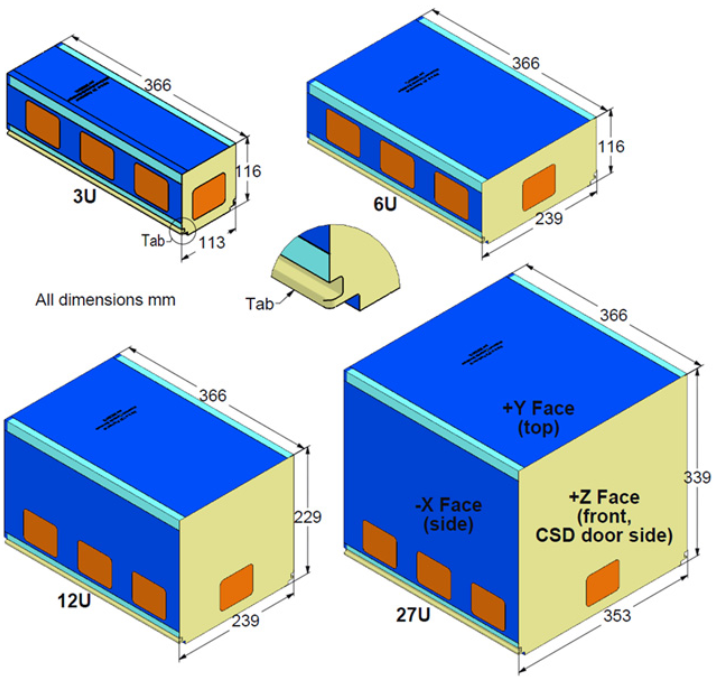
\includegraphics[width=0.60\textwidth]{27U}
					\caption{CubeSat-Größen gemäß der Planetary Systems Corporation \cite{Lettau.}}
					\label{fig:27U}
				\end{figure}
				
				Das Hauptantriebssystem ist der BHT-200 und wird mit dem Treibstoff Iod betrieben. Hier handelt es sich um einen elektrischen Antrieb mit einem TRL-Wert von \num{8} und einem guten leistungspezifischen Schub von \SI{65}{\micro\newton\watt}. Durch das geringe Volumen von \SI{3}{\unit} und der Verwendung von leichten Materialen für die Tankwände bewährt sich Iod als Treibstoff. 
				
Als weiteres Triebwerk wird das chemische Triebwerk Marotta verwendet. Dies dient zur Ausführung von Rendevouz und Docking. Durch die Auslegung der Kaltgaspakete für sehr kleine Satelliten (< \SI{6}{\unit}) weisen sie sehr geringe Schübe auf und erreichen nicht die \SI{0,23}{\newton}. Desto Trotz werden \num{24} Marotta Triebwerke verwendet, um eine 6-DoF-Manövrierfähigkeit zu ermöglichen. Sie weisen im Vergleich zu anderen Kaltgastriebwerken einen hohen $I_{sp}$ Wert von \num{65} auf. Eine Anordnung der \num{24} Marotta Triebwerken befindet sich in der \abb{fig:marotta}. Dieses Triebwerk wird mit Stickstoff betrieben und benötigt zuzüglich von \num{40} \% Sicherheit und der Annahme einer Stabilisierung von einer Sekunde alle \num{10} Orbits eine Gesamttreibstoffmasse von \SI{2,12}{\kilo\gram} \cite{Lettau.}.
				
				\begin{figure}[H]
					\centering
						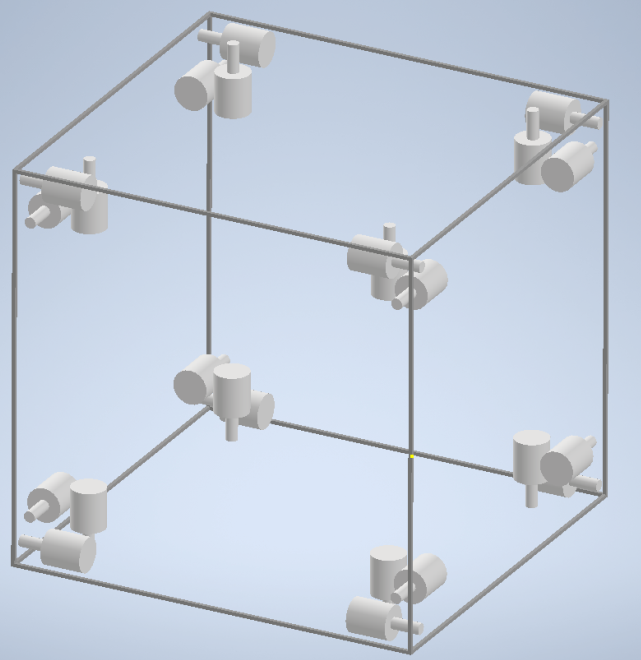
\includegraphics[width=0.30\textwidth]{Marotta}
						\caption{Anordnung der RCS-Triebwerke \cite{Lettau.}}
						\label{fig:marotta}
				\end{figure}
				
				Viele Unternehmen bieten kundenspezifische Lösungen an. Dies wird auch von dem Unternehmen Blue Canyon Technologies für das Solarmodul \SI{6}{\unit}-H triple deployable solar array angeboten. Da es sich um eine zweiflügelige Konfiguration mit einer Grundfläche von \SI{6}{\unit} pro Flügel handelt, wird sie auf eine Grundfläche von \SI{9}{\unit} hoch skaliert, sodass sie auf den \SI{27}{\unit} CubeSat angewendet werden kann. Des Weiteren wird von einer dreiflügeligen Konstellation ausgegangen. Die Vergrößerung der Solaranlage sorgt für eine Steigerung der Nennleistung um \num{50} \%. Weiterhin wird ein Solarpanel auf die obere Grundfläche des CubeSats platziert. Mit allen sieben Solarpanelen erreicht der CubeSat eine Nennleistung von \SI{202}{\watt}. In der \abb{fig:solarpanel} ist eine vereinfachte CAD Darstellung von der Solaranlage zu sehen \cite{Lettau.}.
				
				\begin{figure}[H]
					\centering
						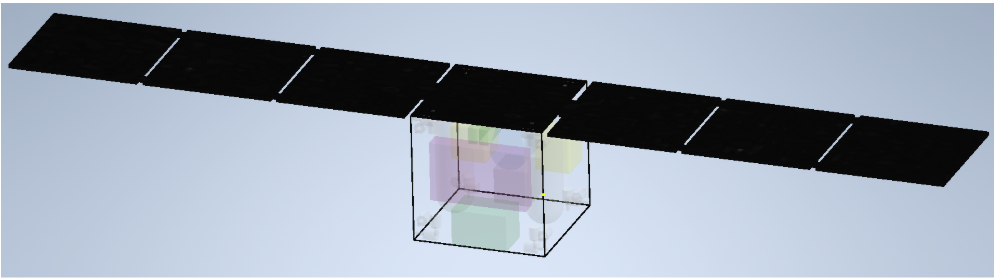
\includegraphics[width=0.60\textwidth]{graphics/Solarpanel.PNG}
						\caption{CAD Darstellung von der Solarkonfiguration \cite{Lettau.}}
						\label{fig:solarpanel}
				\end{figure}
				
				Bei dem Power Management and Distribution System (PMAD-System) ist das NanoAvionics EPS, mit einem TRL von \num{9}, dass geeignetste PMAD-System. Bei dieser Variante ist das besondere, dass ein externes Batteriepack mitgeliefert wird. Die EPS Variante liefert eine Leistung von \SI{175}{\watt} und eine Kapazität von \SI{161}{\watt\hour}. Des Weiteren kann die Batterie skaliert werden, um die Leistungsabgabe zu erhöhen. Unter der Annahme, dass eine relative Navigation von ca. \SI{5}{\kilo\metre} bis zum Andocken erforderlich ist und ein einziger Sensor dies nicht abdecken kann, sind mehrere miteinander kompatible Sensoren notwendig. Als Referenz wird die Mission e.Deorbit-Mission aufgrund von Ähnlichkeiten des Missionsprofils gewählt \cite{Lettau.}.  

				Einen Übersicht über die Komponenten des angenommen Designs ist in der \tab{tab:cubesatdesign} zusehen. Hier werden die Subsysteme mit den dazugehörigen Produkten und deren Mengenangabe aufgelistet. Dies Einordnung orientiert sich an der Struktur der QuSAD Datenbank.
				\begin{table}[H]
				\centering
\begin{tabular}{|l|l|c|}
\hline
\multicolumn{1}{|c|}{Subsystem} & \multicolumn{1}{c|}{Produkt}    	            & Anzahl \\ \hline
Antenne                         & IQW S-Band Dual Patch Antenna                 & 2      \\ \hline
                                & SkyFox Labs piPATCH-MAX (GNSS)                & 2      \\ \hline
Kontroll Board                  & SSTL OBC750 LEO Flight Computer               & 1      \\ \hline
EPS                             & NanoAvionics EPS                              & 1      \\ \hline
Nutzlast \& Verschiedenes       & Vision-based LiDAR Sensor                     & 1      \\ \hline
                                & Crystalspace CAM1U 5 MP (RNS)                 & 2      \\ \hline
                                & Gecko based                                   & 1      \\ \hline
Antrieb                         & Iodine tank                                   & 1      \\ \hline
                                & Nitrogen tank                                 & 1      \\ \hline
                                & Busek BHT-200 Thruster (electric)             & 1      \\ \hline
                                & Marotta Micro-Thruster (chemical)             & 24     \\ \hline
Solar Panel                     & Top/Bottom BCT 9U                             & 1      \\ \hline
                                & BCT 9U Tripple Wing Solar Array Custom (Side) & 1      \\ \hline
                                & BCT SADA Gimbal System                        & 1      \\ \hline
Transceiver                     & IQW Slink-Phy S-Band Transceiver              & 1      \\ \hline
Struktur                        & 27U NanoAvionics Standard Structure (s)       & 1      \\ \hline
Tracker und Sensor               & TY-Space PST3                                 & 2      \\ \hline
                                & NSS Fine Sun Sensor NFSS-411                  & 4      \\ \hline
                                & Sensonor STIM300                              & 1      \\ \hline
                                & SSTL SGR-Ligo                                 & 1      \\ \hline
\end{tabular}
\caption{Angenommenes Design \cite{Lettau.}}
\label{tab:cubesatdesign}
\end{table}
	
						%Hier die Varainte von Max nehmen und kurz beschreiben
				\subsection{Budgetplanung}
				\hfill\emph{(Florian Czorny)}\\
Im folgenden Kapitel wird auf die mittels QuSAD erstellten Budgets für Masse, Volumen und Leistung eingegangen. In QuSAD werden Komponenten in Kategorien eingeteilt. Die Budgets werden mit diesen Kategorien erstellt. Eine Tabelle mit allen Kategorien und den dazugehörigen Komponenten ist in der \tab{tab:cubesatdesign} zu finden. Die Batterie ist im EPS Board integriert und taucht deshalb im Massen- und Volumenbudget nicht auf. Da QuSAD in der Kategorie EPS keinen Eintrag über speicherbare Energie zulässt, wurde die Batterie nur für das Leistungsbudget hinzugefügt. Des weiteren ist zu beachten, dass die Komponenten in den unterschiedlichen Budgets keine einheitliche Farbgebung aufweisen. Einbauvorrichtungen wurden in QuSAD nicht berücksichtigt. Die Abweichungen in den Budgets durch das  zusätzliche Gewicht und Volumen sind davon abhängig, inwiefern die Herstellerangaben den Einbau berücksichtigen.

						\subsubsection{Massenbudget}
Das Massenbudget \abb{fig:masse} zeigt die aktuelle Massenverteilung des Designs an. Die maximal verfügbare Masse ist über eine Angabe in der Strukturkomponente begrenzt. Diese beinhaltet einen Wert für die maximale Gesamtmasse. Die maximale Gesamtmasse des CubeSats wurde mit \SI{50}{\kilogram} angenommen. Das aktuelle Design beansprucht circa \num{57} \% der möglichen Gesamtmasse (\SI{28,5}{\kilogram}). Den größten Teil macht dabei die Antriebsanlage aus. Es gilt zu beachten, dass dieses Budget die Startmasse des CubeSats widerspiegelt. Nach Beginn der Mission ändert sich die Massenverteilung aufgrund des Treibstoffverbrauchs.
										\begin{figure}[H]
											\centering
												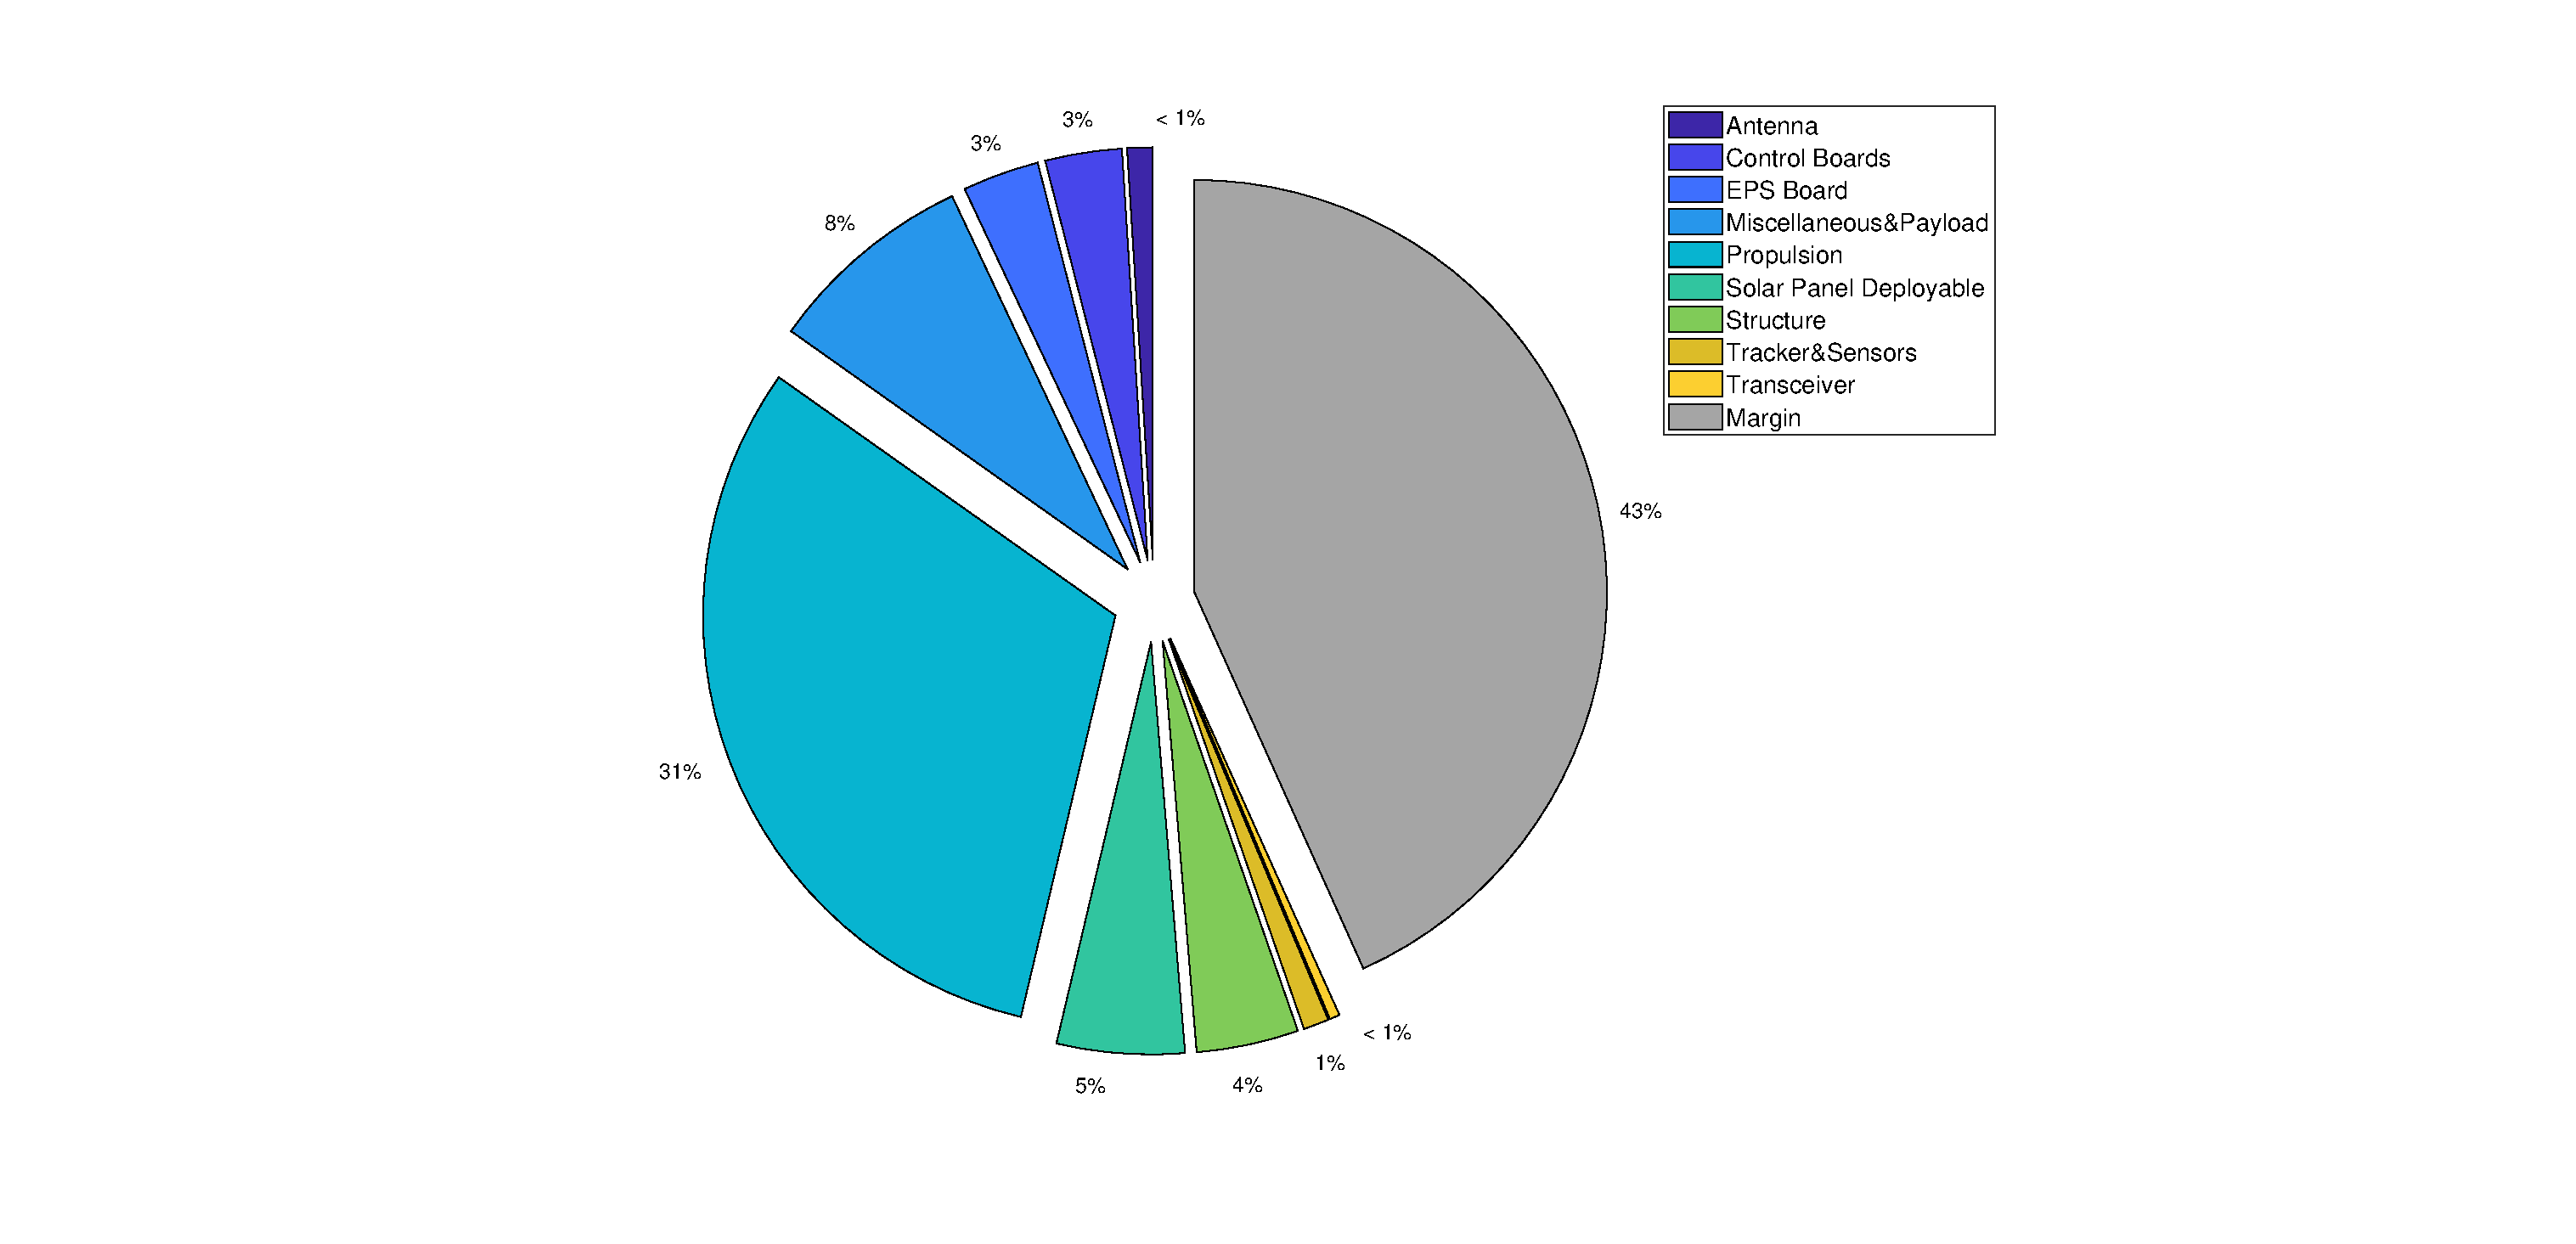
\includegraphics[width=0.90\textwidth]{masse}
											\caption{Massenbudget für das angenommene Design}
											\label{fig:masse}
										\end{figure}
								
						\subsubsection{Volumenbudget}
Das Volumenbudget \abb{fig:volume} gibt einen strukturierten Überblick über die aktuelle Volumenverteilung der ausgewählten Konfiguration, beziehungsweise des Profils in QuSAD. Das maximale verfügbare Volumen bemisst sich an der im Profil befindlichen Strukturkomponente, die über eine Volumenangabe verfügt. Es wurde von einem \SI{27}{\unit} CubeSat mit den Kantenlängen \SI{30 x 30 x 30}{\centi\metre} ausgegangen. Das verfügbare Gesamtvolumen ist bei dieser Annahme im Gegensatz zur Masse jedoch zu circa \num{97} \% ausgelastet. Es fällt auf, dass nahezu alle Kategorien einen größeren Volumenanteil als Massenanteil aufweisen. Das größte Volumen nimmt, ähnlich wie beim Massenbudget die Antriebsanlage ein. Sie macht jedoch der Treibstofftanks über die Hälfte des Gesamtvolumens aus. Es sollte beachtet werden, dass aufgrund des geringen Freiraums kaum Sicherheiten möglich sind.
		
										\begin{figure}[H]
											\centering
												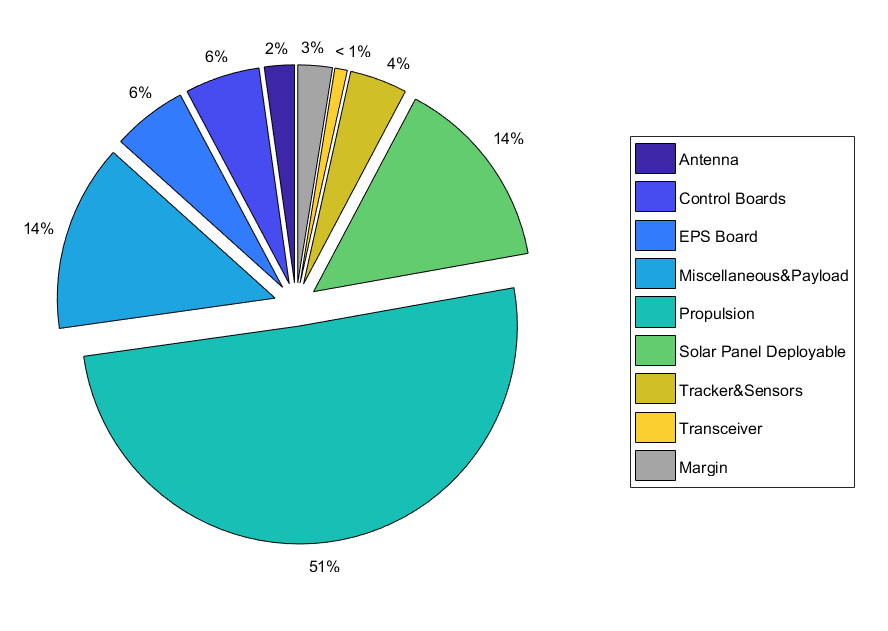
\includegraphics[width=0.90\textwidth]{volume}
											\caption{Volumenbudget für das angenommene Design}
											\label{fig:volume}
										\end{figure}
								
						\subsubsection{Leistungsbudget}
Das Leistungsbudget \abb{fig:power} gibt einen Überblick über den Verbrauch der verschiedenen Komponenten. Es gibt die Entladung der Batterie auf der Schattenseite der Erde wieder (Req. Battery Power) und wie in den anderen Budgets die Spanne zur Systemuntauglichkeit (Margin). Der Antrieb nimmt mit \num{32} \% insgesamt den größten Anteil des Energieverbrauchs ein.
				
										\begin{figure}[H]
											\centering
												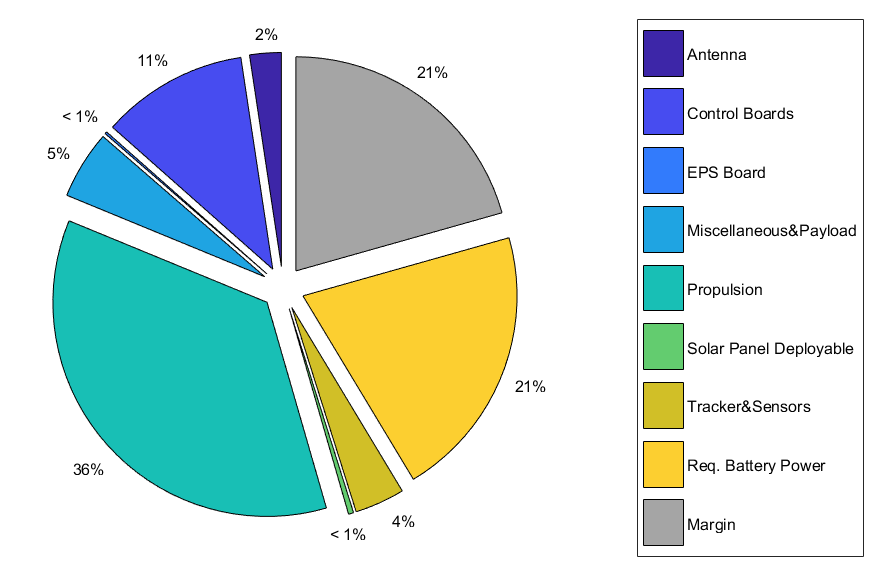
\includegraphics[width=0.90\textwidth]{power}
											\caption{Energiebudget für das angenommene Design}
											\label{fig:power}
										\end{figure}
Um das Leistungsbudget zu erstellen, muss die Höhe der Umlaufbahn und der Brennwinkel $\beta$ angegeben werden (\abb{fig:power1}). Diese wurden mit \SI{1150}{\kilo\metre} und 0\textdegree{} angenommen (\tab{tab:cubesatdesign}).  Das Programm ermittelt für diese Parameter direkt die Zeit einer Orbitperiode und die dazugehörige Licht- und Schattenzeit. Mit den Angenommenen Parametern ergibt sich eine Umlaufdauer von \num{108,34} Minuten bei einer Sonnenzeit von \num{73,48} Minuten. Die im Designe enthaltenen Solarpanele müssen einer Position am CubeSat zugeordnet werden.
Nachdem die maximale Missionsdauer angegeben wurde kann die Energieerzeugung während einer Erdumrundung berechnet werden (\abb{fig:power3} und \abb{fig:power4}). Dabei wird mit einer  Verschlechterung der Energieerzeugung von \num{3} \% pro Missionsjahr gerechnet. Diese spiegelt sich dann in der angepassten Leistung der Solarpanele wieder. Das Programm bezieht außerdem die verschiedenen Beläuchtungsfälle der Solarzellen bei verschiedenen Sonnenwinkeln $\alpha$ ein. Um eine Gesamtenergie berechnen zu können,  werden Wahrscheinlichkeiten für die verschiedenen Beläuchtungsfälle angenommen. Die endgültige Leistung der Konfiguration beläuft sich auf \SI{143,144}{\watt}. Bei einer Sonnenzeit von \num{73,48} Minuten ergeben sich \SI{175,27}{\watt\hour} pro Erdumrundung. 
			
			\begin{figure}[H]
				\centering
					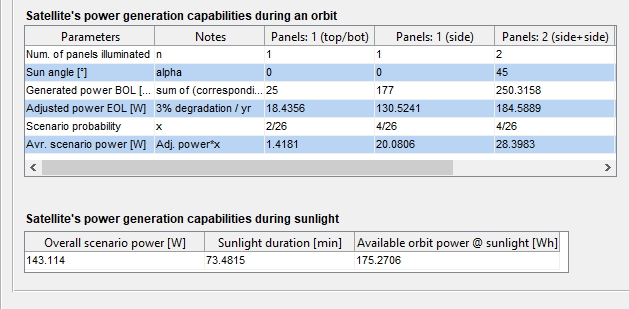
\includegraphics[width=0.70\textwidth]{graphics/power3.png}
				\caption{QuSAD: Energieerzeugung pro Orbit 1}
				\label{fig:power3}
			\end{figure}
			
			\begin{figure}[H]
				\centering
					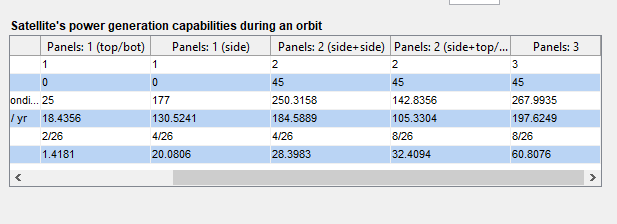
\includegraphics[width=0.70\textwidth]{graphics/power4.PNG}
				\caption{QuSAD: Energieerzeugung pro Orbit 2}
				\label{fig:power4}
			\end{figure}
Da das Haupttriebwerk und das RCS-System nicht dauerhaft betrieben werden, muss für diese Komponenten eine Prozentuale Brenndauer angegeben werden. Die mit den getroffenen Annahmen über die Brenndauer veränderten Werte  (\tab{tab:cubesatdesign}) können manuell in QuSAD geändert werden. Für das Haupttriebwerk wurden \num{16,1} \% und Das RCS-System \num{0,001} \% Nutzungszeit angenommen. Bei den anderen Komponenten wird von einem dauerhaften Betrieb ausgegangen. Der Energieverbrauch jeder Komponente pro Orbit wird direkt angezeigt. (\abb{fig:power5})
			
			\begin{figure}[H]
				\centering
					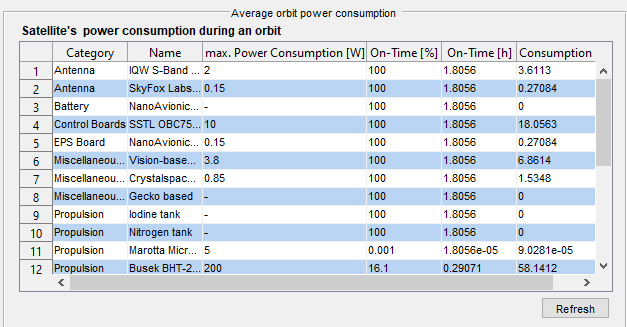
\includegraphics[width=0.70\textwidth]{graphics/power5.png}
				\caption{QuSAD: Energieverbrauch pro Orbit}
				\label{fig:power5}
			\end{figure}
Die von QuSAD angenommenen Werte zur Bestimmung des Energieüberschusses sind in  \abb{fig:power6} zusammengefasst. Es kann genau bestimmt werden wie viel Energie die Konfiguration während der Sonnen- und Schattenperiode zur Verfügung hat und wie viel davon verbraucht wird. Aus dem Budget ist dann der Anteilige Verbrauch der 
einzelnen Komponenten ersichtlich.

			
			\begin{figure}[H]
				\centering
					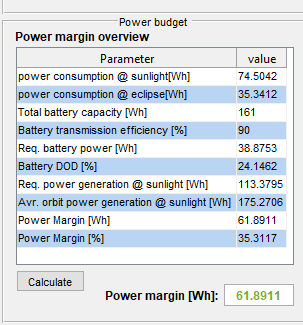
\includegraphics[width=0.45\textwidth]{graphics/power6.png}
				\caption{QuSAD: Überblick Energieüberschuss}
				\label{fig:power6}
			\end{figure}
Zur Berechnung des Budgets wird eine Batterieeffizienz von \num{90} \% angenommen. Der Wert “Power margin” gibt den Energieüberschuss eines Orbits in Wh an (\abb{fig:power6}). Das Budget in \abb{fig:power} stellt den Zustand des CubeSats nach der angegebenen Missionsdauer in \abb{fig:power2} dar. Die Energieproduktion pro Orbit sinkt mit dem Fortlaufen der  Mission. Somit ist der Energieüberschuss bei Missionsstart deutlich höher. 			
			
			
			
			\section{Auswertung und Optimierung des Designs}
Die Auswertung der Ergebnisse zeigt, dass bei der Masse eine Steigerung von \SI{21,5}{\kilogram} (\num{43} \%) und bei dem Volumen hingegen lediglich eine Steigerung von \SI{815}{\centi\metre\cubed} (\num{3} \%) gemäß QuSAD zulässig ist. Hier lässt sich feststellen, dass das Programm von dem Gesamtvolumen \SI{27000}{\centi\metre\cubed} ausgeht, wobei das maximal verfügbare Volumen bei einem \SI{34 x 35 x 36}{\centi\metre} großen Satelliten mit \SI{42840}{\centi\metre\cubed} festgelegt ist \cite{Lettau.}. Dies weist eine Differenz von \num{38,88} \% auf. Demzufolge muss bei der Konfiguration ein verfügbares Volumen von \num{41,88} \% vorhanden sein. Rückwirkend lässt sich feststellen, dass beim einpflegen der Daten ein zulässiges Gesamtvolumen manuell eingetragen werden muss, andernfalls orientiert sich das Programm an der Dimension, die in diesem Fall mit \SI{27}{\unit} ein Volumen von \SI{27000}{\centi\metre\cubed} aufweist. An dieser Stelle muss beachtet werden, dass bei vielen Komponenten keine genauen Angaben bezüglich der Masse und des Volumens gegeben waren und dementsprechend durch Vergleich mit näherungsweise ähnlichen Systemen oder Aufwärtsskalierung die Werte bestimmt wurden. Zusätzlich kommt bei dem Massen Budget hinzu, dass die Software keine Einbauvorrichtungen berrücksichtigt. Demnach würde sich die verfügbare Spanne für Masse als auch Volumen senken.  Bei dem Leistungsbudget muss beachtet werden, dass der erhöhte Verbrauch während des RDVDO nicht berücksichtigt wird. An dieser Stellen empfiehlt sich eine weitere Untersuchung. Den Ergebnissen zufolge lässt sich die betrachtete Mission mit dem aktuellen Stand des Designs durchführen und demzufolge ist bislang keine Optimierung erforderlich. Da in dem aktuellen Entwurf viele Unsicherheiten vorhanden sind und einige Aspekte durch das Leistungsbudget nicht beachtet worden sind, wie die Tankmasse, könnte eine Optimierung nach der Missionsanalyse notwendig sein. 
